% Appendix C: Additional Figures and Diagnostic Plots
% Focus: Placeholders for supplemental tables and figures (e.g. Pearson/Spearman heatmaps, full distributions, UMAPs).
% Document Feeds: docs/reduced_metric_core.md, docs/visualization.md
% TODO: Embed secondary plots that do not fit in the main chapters.

\label{app:additional-figures}

\noindent This appendix compiles supplemental diagnostic plots, secondary correlation matrices, and granular subfield UMAP maps that provide deeper contextual verification of the results discussed in the main body.

\section{Centroid-Embedding Clustering Sensitivity}

Chapter~9 clusters subfields by morphology: the eleven robust-scaled profile metrics derived from original SPECTER2 space. As a sensitivity check, the analysis was repeated with a different representation. For each analysis subfield \(s\), a semantic-location centroid was computed as
\[
\bar{z}_s=\frac{1}{n_s}\sum_{i\in s}z_i,
\]
where paper embeddings \(z_i\) were L2-normalized before averaging and each resulting centroid \(\bar{z}_s\) was L2-normalized again before clustering. This check therefore asks whether subfields separate more clearly by semantic location than by morphology.

The centroid exploration covered Ward hierarchical clustering, average-link hierarchical clustering, \(k\)-means, and nearest-neighbor spectral clustering for \(k=3,\ldots,10\). HDBSCAN was not available in the active environment and was not forced. The best balanced centroid solution used average linkage with cosine distance at \(k=3\), with silhouette \(=0.236\) and cluster sizes \(157\), \(60\), and \(24\). Agreement with the selected morphology typology was low (ARI \(=0.085\), AMI \(=0.084\)), while alignment with OpenAlex domains was higher (ARI \(=0.279\), AMI \(=0.471\)). A directly comparable Ward \(k=5\) centroid solution had silhouette \(=0.156\), AMI \(=0.095\) against the morphology typology, and AMI \(=0.569\) against domains.

The result does not overturn the Chapter~9 interpretation. It indicates that semantic location carries a stronger domain/topic structure than morphology, but it does not turn either representation into a sharply partitioned space. The low agreement between centroid clusters and morphology typologies is useful: the five typologies in Chapter~9 describe recurrent shape profiles, not hidden topic clusters or replacements for the OpenAlex hierarchy.

\begin{figure}[H]
\centering
\caption[Centroid-embedding clustering sensitivity]{Centroid-embedding clustering sensitivity. Panel A repeats the selected Ward \(k=5\) morphology typology in robust-scaled eleven-metric PCA space. Panel B projects L2-normalized subfield centroid embeddings into PCA space and colors the selected balanced average-link cosine solution at \(k=3\). Centroids are computed from L2-normalized paper-level SPECTER2 vectors; distances express semantic location rather than morphology. PCA is used only for visualization and is not used to assign either morphology typologies or centroid clusters.}
\label{fig:centroid_embedding_clustering_sensitivity}
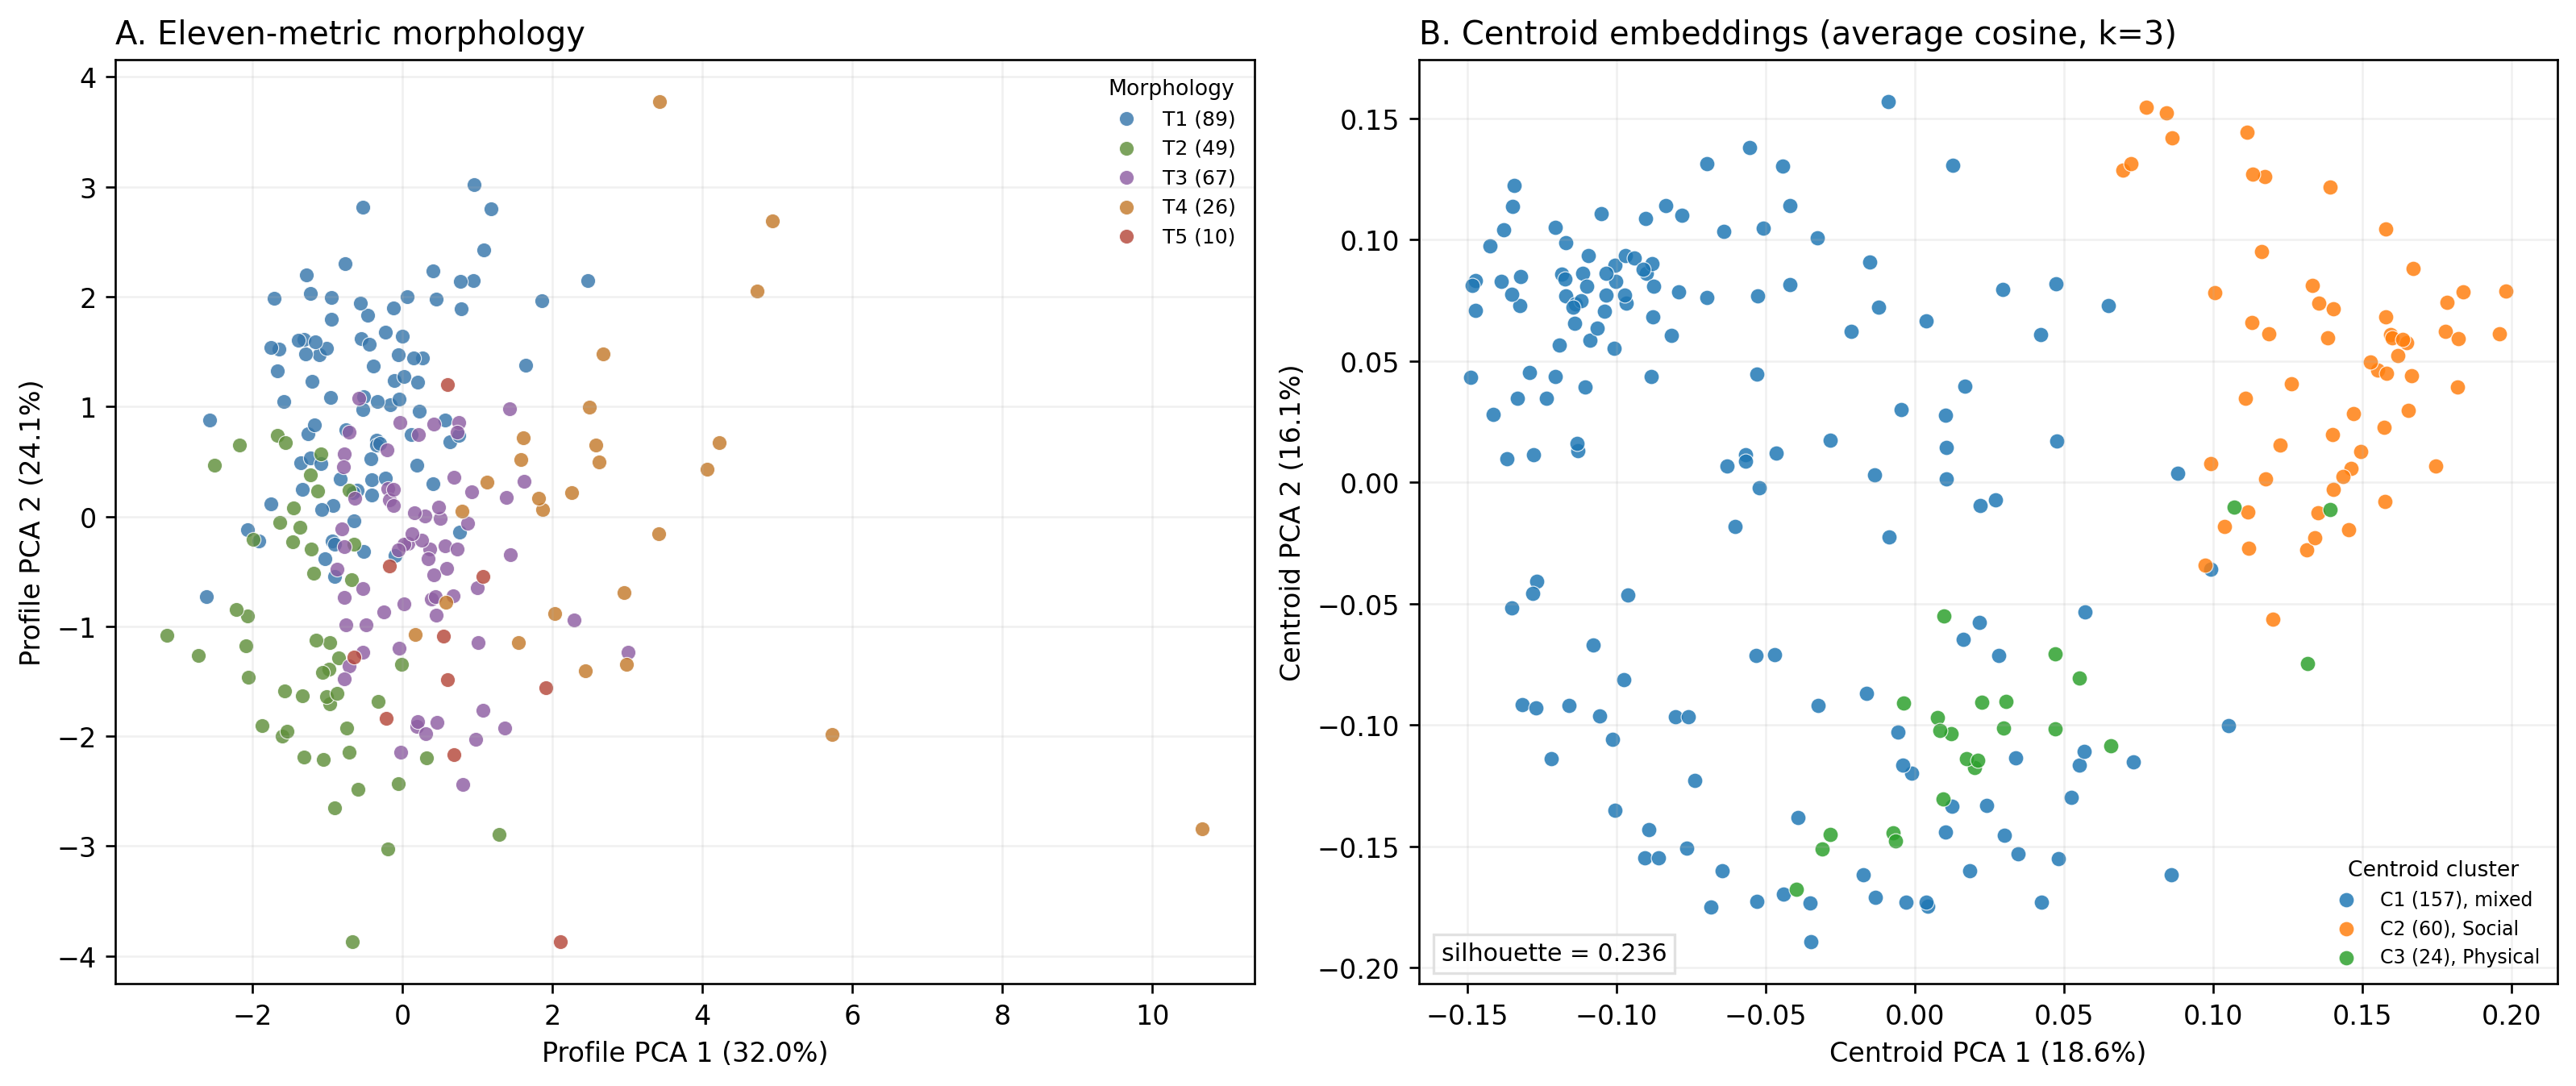
\includegraphics[width=\textwidth]{figures/fig_09_centroid_embedding_clustering_sensitivity.png}
\end{figure}

\section{Temporal-Trajectory and Hybrid Clustering Sensitivity}

Two further sensitivity checks ask whether the weak morphology typology changes when the representation is altered. The temporal-trajectory check clusters subfields by change in the eight windowed structural metrics across the five thesis windows. Because one subfield lacks a completed 2000--2004 window, this check uses 240 complete trajectories. Four representations were tested: first--last change vectors, linear slope vectors, full window-by-metric trajectories, and a dynamic summary combining changes, slopes, volatility, and centroid-path movement.

The best balanced temporal solution uses average-link hierarchical clustering on correlation distances between the eight-metric slope vectors, with \(k=4\), silhouette \(=0.396\), and cluster sizes \(93\), \(58\), \(54\), and \(35\). Its mean subsample ARI is \(0.725\), so this dynamic partition is more stable than the full-period morphology typology. It is not, however, the same object: agreement with the Chapter~9 morphology typology is low (AMI \(=0.048\)), and agreement with OpenAlex domains is also low (AMI \(=0.093\)). The groups are better read as dynamic tendencies: one cluster becomes more compact and locally denser; another expands in centroid and nearest-neighbor distance while hubness falls; a third loosens local neighborhoods while local unevenness declines; and a smaller group gains dimensionality and hub concentration.

The hybrid check combines semantic location with morphology. Two families were tested: concatenating balanced morphology profiles with reduced centroid principal components, and weighted distance matrices \(D_{\mathrm{hybrid}}=\alpha D_{\mathrm{centroid}}+(1-\alpha)D_{\mathrm{morphology}}\) for \(\alpha\in\{0.25,0.50,0.75\}\). The best balanced hybrid solution uses spectral clustering on the \(\alpha=0.75\) hybrid distance matrix, with \(k=3\), silhouette \(=0.247\), and cluster sizes \(91\), \(77\), and \(73\). It is highly stable under subsampling (mean ARI \(=0.951\)), but it aligns much more with centroid/domain structure than with morphology: AMI is \(0.591\) against OpenAlex domains, \(0.505\) against centroid clusters, and only \(0.092\) against the morphology typology. The hybrid result therefore confirms that semantic location dominates once it receives substantial weight.

These checks add nuance rather than a replacement typology. Temporal trajectories are useful for Chapter~7-style questions about how morphology changes; hybrid clusters are useful for showing how quickly semantic location reconstructs broad disciplinary structure. The Chapter~9 typology remains the appropriate summary for full-period morphology profiles.

\begin{figure}[H]
\centering
\caption[Temporal and hybrid clustering sensitivity]{Temporal and hybrid clustering sensitivity. Panel A projects the selected temporal slope-vector solution into PCA space and colors subfields by dynamic cluster. Panel B shows the OpenAlex domain composition of the selected hybrid centroid--morphology solution. The temporal projection is for visualization only; clustering uses standardized slope vectors. The hybrid solution uses a weighted distance matrix, not PCA or UMAP coordinates.}
\label{fig:temporal_hybrid_clustering_sensitivity}
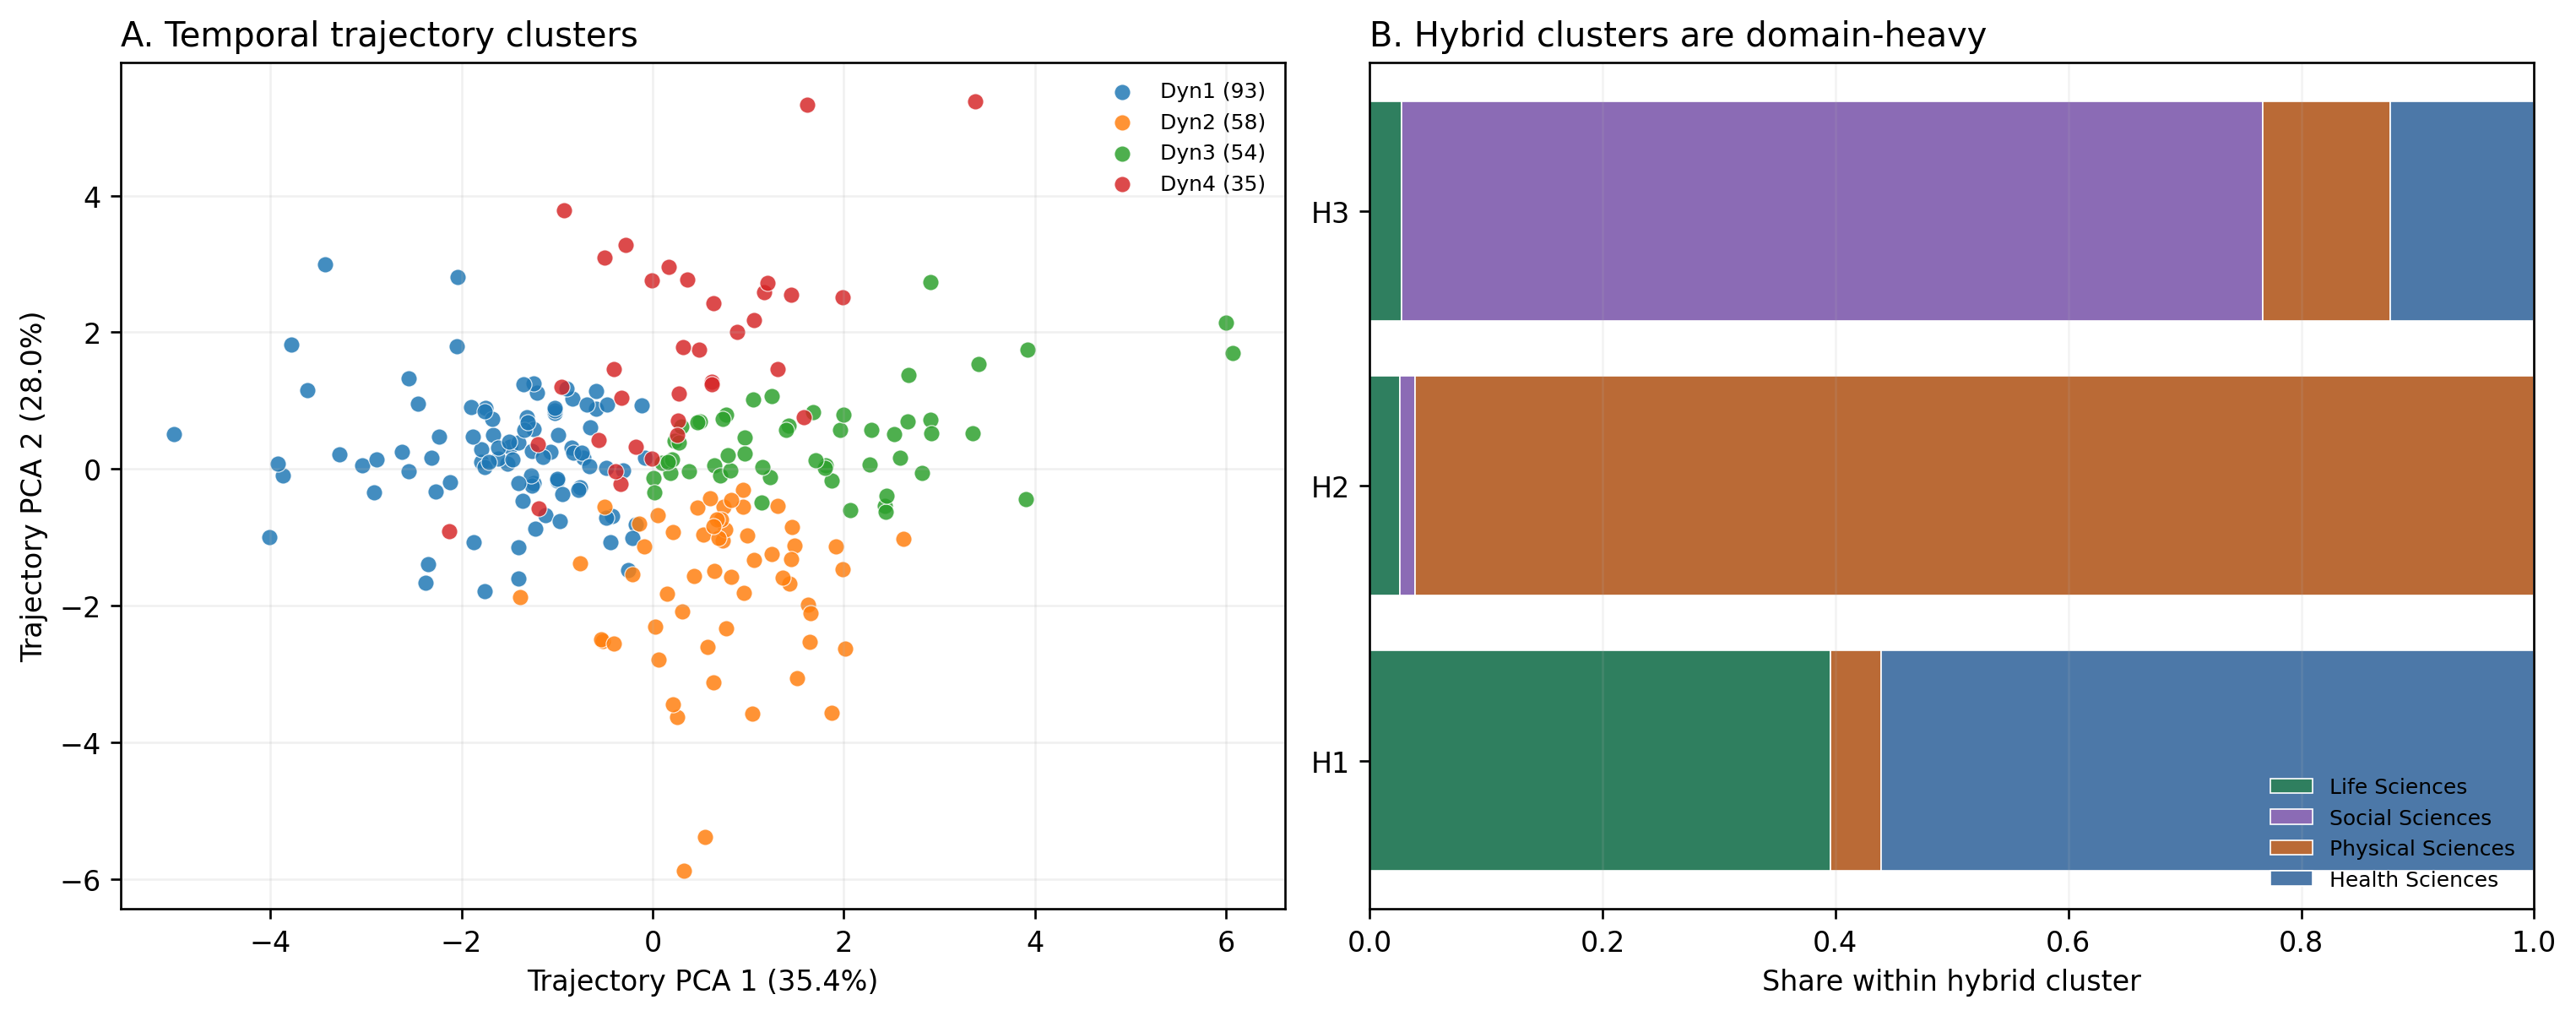
\includegraphics[width=\textwidth]{figures/fig_c_temporal_hybrid_clustering_sensitivity.png}
\end{figure}

% TODO: Include Spearman and Pearson metric correlation heatmaps.
% TODO: Include metric distribution histograms across all subfields.
% TODO: Include granular smooth density UMAP subfield panels for inspection.
